\documentclass[9pt,aspectratio=169,xcolor=table]{beamer}

%~~~~~~~~~~~~~~~~~~~~~~~~~~~~~~~~~~~~~~~~~~~~~~~~~~~~~~~~~~~~~~~~~~~~~~~~~~~~~~
% Use roboto Font (recommended)
\usepackage[sfdefault]{roboto}
\usepackage[utf8]{inputenc}
\usepackage[T1]{fontenc}
%~~~~~~~~~~~~~~~~~~~~~~~~~~~~~~~~~~~~~~~~~~~~~~~~~~~~~~~~~~~~~~~~~~~~~~~~~~~~~~

%~~~~~~~~~~~~~~~~~~~~~~~~~~~~~~~~~~~~~~~~~~~~~~~~~~~~~~~~~~~~~~~~~~~~~~~~~~~~~~
% Define where theme files are located. ('/styles')
\usepackage{styles/fluxmacros}
\usefolder{styles}
% Use Flux theme v0.1 beta
% Available style: asphalt, blue, red, green, gray
% "red" is the closest built-in style to maroon; its exact colours are
% overridden with a true maroon palette just below, after the theme loads.
\usetheme[style=red]{flux}
%~~~~~~~~~~~~~~~~~~~~~~~~~~~~~~~~~~~~~~~~~~~~~~~~~~~~~~~~~~~~~~~~~~~~~~~~~~~~~~

%~~~~~~~~~~~~~~~~~~~~~~~~~~~~~~~~~~~~~~~~~~~~~~~~~~~~~~~~~~~~~~~~~~~~~~~~~~~~~~
% SKEE1033 maroon palette override.
% The flux theme's colortheme defines primaryLight/primary/secondary/tertiary
% as plain \definecolor calls (not \providecolor), so simply redefining them
% here, AFTER \usetheme, wins -- xcolor allows redefinition and every
% \setbeamercolor in beamercolorthemeflux.sty was already evaluated against
% these names, so the redefinition propagates everywhere automatically.
\definecolor{primaryLight}{HTML}{9B2242} % lighter maroon -- headers, accents
\definecolor{primary}{HTML}{7B1E3A}      % core maroon -- titles, block headers
\definecolor{secondary}{HTML}{3A5A6B}    % muted teal -- complementary accent
\definecolor{tertiary}{HTML}{8C6A3F}     % warm bronze -- example/third accent
%~~~~~~~~~~~~~~~~~~~~~~~~~~~~~~~~~~~~~~~~~~~~~~~~~~~~~~~~~~~~~~~~~~~~~~~~~~~~~~

%~~~~~~~~~~~~~~~~~~~~~~~~~~~~~~~~~~~~~~~~~~~~~~~~~~~~~~~~~~~~~~~~~~~~~~~~~~~~~~
% Extra packages
\usepackage{booktabs}
\usepackage{colortbl}
\usepackage{ragged2e}
\usepackage{amssymb}
\usepackage{multirow}
\usepackage{tikz}
\usetikzlibrary{arrows.meta, positioning, fit, backgrounds, calc, shapes.geometric}
\setbeamertemplate{itemize items}[square]
\usepackage[scaled=.92]{beramono}
\usepackage{listings}
\usepackage{array}
% Table striping: odd rows white, even rows very light gray.
\definecolor{stripe}{gray}{0.94}
\newcommand{\striped}{\rowcolors{1}{white}{stripe}}
%~~~~~~~~~~~~~~~~~~~~~~~~~~~~~~~~~~~~~~~~~~~~~~~~~~~~~~~~~~~~~~~~~~~~~~~~~~~~~~

%~~~~~~~~~~~~~~~~~~~~~~~~~~~~~~~~~~~~~~~~~~~~~~~~~~~~~~~~~~~~~~~~~~~~~~~~~~~~~~
% Code listing style (lightweight analogue of the book's skpython style).
% This course is Python-only, so Python is set as the lstlisting default via
% \lstset below -- every \begin{lstlisting} needs no language=... of its own.
\definecolor{codebg}{HTML}{FBF2F4}
\definecolor{codegreen}{rgb}{0,0.45,0}
\definecolor{codestring}{rgb}{0.58,0.1,0.2}
\lstdefinestyle{skpython}{
    basicstyle=\ttfamily\footnotesize,
    keywordstyle=\color{primary}\bfseries,
    commentstyle=\itshape\color{codegreen},
    stringstyle=\ttfamily\color{codestring},
    backgroundcolor=\color{codebg},
    breaklines=true,
    keepspaces=true,
    showspaces=false,
    showstringspaces=false,
    frame=single,
    rulecolor=\color{primary!40},
    numbers=none,
}
\lstset{language=Python, style=skpython}
%~~~~~~~~~~~~~~~~~~~~~~~~~~~~~~~~~~~~~~~~~~~~~~~~~~~~~~~~~~~~~~~~~~~~~~~~~~~~~~

%~~~~~~~~~~~~~~~~~~~~~~~~~~~~~~~~~~~~~~~~~~~~~~~~~~~~~~~~~~~~~~~~~~~~~~~~~~~~~~
% TikZ block styles for the computation-cycle and control-structure diagrams
\definecolor{cycfill}{HTML}{F3DCE4}
\definecolor{cycline}{HTML}{7B1E3A}
\definecolor{cycdofill}{HTML}{E8EEF0}
\definecolor{cycdoline}{HTML}{3A5A6B}
\tikzset{
  cycstep/.style = {font=\sffamily\small, align=center, rounded corners=2pt,
                     draw=cycline, fill=cycfill, line width=0.7pt,
                     minimum height=7mm, minimum width=20mm, inner sep=3pt},
  cycdo/.style   = {cycstep, fill=cycdofill, draw=cycdoline},
  flow/.style    = {-{Stealth[length=2mm]}, thick, draw=cycline},
}
%~~~~~~~~~~~~~~~~~~~~~~~~~~~~~~~~~~~~~~~~~~~~~~~~~~~~~~~~~~~~~~~~~~~~~~~~~~~~~~

%%%%%%%%%%%%%%%%%%%%%%%%%%%%%%%%%%%
%% SECTION SEPARATOR (ToC recap) %%
%%%%%%%%%%%%%%%%%%%%%%%%%%%%%%%%%%%
\AtBeginSection[]
{
{
    \setbeamercolor{background canvas}{bg=primaryLight!6}
    \begin{frame}[plain]
        \frametitle{Table of Contents}
        \tableofcontents[currentsection]
    \end{frame}
}
}
%%%%%%%%%%%%%%%%%%%%%%%%%%%%%%%%%%%

%~~~~~~~~~~~~~~~~~~~~~~~~~~~~~~~~~~~~~~~~~~~~~~~~~~~~~~~~~~~~~~~~~~~~~~~~~~~~~~
% Information
\title{Interpolation, Curve Fitting and Calibration}
\subtitle{\emph{Engineering Computation with Python} --- Chapter 12}
\author{Mun\'{i}m Zabidi}
\institute{\color{primary}Faculty of Electrical Engineering, Universiti Teknologi Malaysia}
\date{\today}
\titlegraphic{assets/logoutmwhite.png}
%~~~~~~~~~~~~~~~~~~~~~~~~~~~~~~~~~~~~~~~~~~~~~~~~~~~~~~~~~~~~~~~~~~~~~~~~~~~~~~

\begin{document}

\titlepage

\begin{frame}{Table of Contents}
    \tableofcontents
\end{frame}

%===============================================================================
\section{Interpolation vs.\ Curve Fitting}
%===============================================================================

\begin{frame}{Two Questions About Discrete Data}
    \leavevmode
    Measurements are taken at discrete points, but engineering questions
    rarely land exactly on one of them. This chapter covers two
    complementary answers.

    \vspace{3mm}
    \begin{columns}[t]
        \begin{column}{.5\textwidth}
            \begin{block}{Interpolation}
                \small Estimates values \alert{between} measured points.
                Passes exactly through every known point.
            \end{block}
        \end{column}
        \begin{column}{.5\textwidth}
            \begin{block}{Curve Fitting}
                \small Finds the single model that best describes a whole
                \alert{noisy} dataset. Does not need to pass through any
                particular point.
            \end{block}
        \end{column}
    \end{columns}

    \vspace{3mm}
    \begin{alertblock}{The choice that matters}
        Clean, exact data $\to$ interpolate. Noisy, scattered measurements
        $\to$ fit. Curve fitting is the basis of \textbf{sensor
        calibration}.
    \end{alertblock}
\end{frame}

\begin{frame}{Interpolation Versus Curve Fitting}
    \leavevmode
    \small
    \begin{table}
    \centering
    \begin{tabular}{p{.47\textwidth}p{.47\textwidth}}
        \toprule
        \textbf{Interpolation} & \textbf{Curve Fitting} \\
        \midrule
        Computes missing values between two known points. &
        Converts data points into a mathematical equation. \\[2mm]
        Original data points are preserved --- the interpolant passes
        exactly through them. &
        The fitted curve does not need to pass through the original data
        points. \\
        \bottomrule
    \end{tabular}
    \end{table}
\end{frame}

%===============================================================================
\section{1-D Interpolation in Python}
%===============================================================================

\begin{frame}[fragile]{The \texttt{interp1d} Syntax}
    \leavevmode
    One-dimensional interpolation in SciPy follows a consistent pattern:
    build an interpolating function once, then call it at any query
    points.

\begin{lstlisting}
from scipy.interpolate import interp1d

# Define the interpolation function
f = interp1d(x, v, kind=method)

# Interpolated values at xq
vq = f(xq)
\end{lstlisting}

    \vspace{2mm}
    \small
    \texttt{numpy.interp()} does the same job for the linear case alone,
    with no object to build first.
\end{frame}

\begin{frame}{\texttt{interp1d} Parameters}
    \leavevmode
    \small
    \begin{table}
    \centering
    \begin{tabular}{p{.18\textwidth}p{.74\textwidth}}
        \toprule
        \textbf{Parameter} & \textbf{Description} \\
        \midrule
        \texttt{x} & Sample points (array-like). \\
        \texttt{v} & Corresponding values at the sample points. \\
        \texttt{xq} & Points at which to evaluate the interpolation. \\
        \texttt{method} & \texttt{'linear'}, \texttt{'nearest'},
        \texttt{'cubic'}, etc. \\
        \texttt{vq} & The interpolated values at \texttt{xq}. \\
        \bottomrule
    \end{tabular}
    \end{table}
\end{frame}

\begin{frame}{The Linear Interpolation Formula}
    \leavevmode
    Every linear-interpolation call, under the hood, evaluates one
    formula. Given two known points $(x_0, y_0)$ and $(x_1, y_1)$, the
    value $y$ at a query point $x$ with $x_0 \le x \le x_1$ is

    \[
    y = y_0 + (x - x_0)\,\frac{y_1 - y_0}{x_1 - x_0}.
    \]

    \vspace{2mm}
    \begin{block}{What this is, geometrically}
        A straight line fitted \alert{between the two known points},
        evaluated at $x$. This is exactly what \texttt{numpy.interp()}
        and \texttt{interp1d(..., kind='linear')} compute.
    \end{block}
\end{frame}

\begin{frame}{Three Interpolation Methods}
    \leavevmode
    \small
    \begin{table}
    \centering
    \begin{tabular}{lp{.52\textwidth}p{.16\textwidth}}
        \toprule
        \textbf{Method} & \textbf{Description} & \textbf{Min.\ Points} \\
        \midrule
        \texttt{nearest} & Steps to the value of the nearest data point. &
        2 \\
        \texttt{linear} & Straight lines connect the points. & 2 \\
        \texttt{cubic} & Piecewise cubic spline. & 4 \\
        \bottomrule
    \end{tabular}
    \end{table}

    \vspace{3mm}
    \begin{alertblock}{Choosing a method is choosing an assumption}
        \texttt{nearest} assumes the signal holds its value until the
        next sample; \texttt{linear} assumes constant rate of change;
        \texttt{cubic} assumes smoothness. None of these is automatically
        correct --- the right choice depends on the physics being
        measured.
    \end{alertblock}
\end{frame}

\begin{frame}[fragile]{Worked Example: Comparing Interpolation Methods}
    \leavevmode
    The same four points, interpolated three different ways:

\begin{lstlisting}
x = np.array([0, 1, 1, 0])
n1 = np.arange(0, 4)
n2 = np.arange(0, 3.2, 0.2)

xnearest = interp1d(n1, x, kind='nearest')
xlinear  = interp1d(n1, x, kind='linear')
xspline  = interp1d(n1, x, kind='cubic')

plt.plot(n1, x, 'o', label='Original Points')
plt.plot(n2, xnearest(n2), '-x', label='Nearest')
plt.plot(n2, xlinear(n2),  ':s', label='Linear')
plt.plot(n2, xspline(n2),  '--*', label='Spline')
\end{lstlisting}
\end{frame}

\begin{frame}{Reading the Comparison Plot}
    \leavevmode
    \begin{center}
    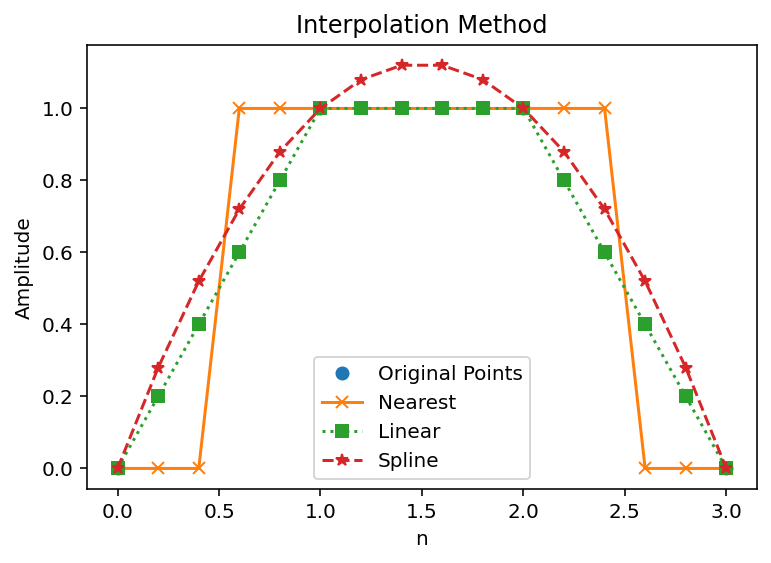
\includegraphics[height=0.56\textheight]{../images/chapter12/interpolation_methods_comparison.png}
    \end{center}

    \vspace{1mm}
    \small
    \textbf{Nearest} produces a step-like response. \textbf{Linear}
    produces straight-line segments with visible corners. \textbf{Spline}
    produces a smooth curve --- but notice it \alert{overshoots} above 1
    and below 0, values the original data never contained.
\end{frame}

%===============================================================================
\section{Worked Example: The API Haze Crisis}
%===============================================================================

\begin{frame}{The Air Pollutant Index}
    \leavevmode
    The API describes air quality from readings at monitoring stations,
    adopted by Malaysia's Department of Environment in 1996 (based on the
    US-EPA Pollutant Standards Index).

    \vspace{3mm}
    \begin{block}{By the way: understanding the API scale}
        \small
        \begin{center}
        \begin{tabular}{cl}
            \toprule
            \textbf{API Range} & \textbf{Health Status} \\
            \midrule
            0--50 & Good \\
            51--100 & Moderate \\
            101--200 & Unhealthy \\
            201--300 & Very Unhealthy \\
            301+ & Hazardous \\
            \bottomrule
        \end{tabular}
        \end{center}
    \end{block}
\end{frame}

\begin{frame}{The Problem: A Haze Crisis}
    \leavevmode
    During a haze crisis, API readings are recorded at five stations
    along the route from Kulai to Johor Bahru:

    \vspace{2mm}
    \small
    \begin{table}
    \centering
    \begin{tabular}{lccccc}
        \toprule
        \textbf{Station} & Kulai & Senai & Skudai & Perling & JB \\
        \midrule
        Distance (km) & 0 & 6 & 15 & 23 & 30 \\
        API value & 100 & 180 & 199 & 280 & 310 \\
        \bottomrule
    \end{tabular}
    \end{table}

    \vspace{3mm}
    \begin{alertblock}{The question}
        What is the API at a location with \alert{no sensor} --- say,
        kilometre 10? Assume the API varies linearly between neighbouring
        stations.
    \end{alertblock}
\end{frame}

\begin{frame}[fragile]{Building the Interpolation Function}
    \leavevmode
    A helper normalizes the input shape first:

\begin{lstlisting}
arraykm = np.atleast_1d(km)
\end{lstlisting}
    \small
    This accepts a single integer, a list, or a NumPy array uniformly
    --- one code path, no type-checking branches.

\begin{lstlisting}
def API_interpolation(km):
    distances  = np.array([0, 6, 15, 23, 30])
    api_values = np.array([100, 180, 199, 280, 310])
    full_distances = np.arange(0, 31, 1)
    interpolated_api = np.interp(full_distances,
                                  distances, api_values)
    km = np.atleast_1d(km)
    result = {}
    for k in km.astype(int):
        result[k] = round(interpolated_api[k], 2)
    return result
\end{lstlisting}
\end{frame}

\begin{frame}[fragile]{Calling It Three Ways}
    \leavevmode
\begin{lstlisting}
API_interpolation(10)                    # Single integer
API_interpolation([3, 8, 11, 26])        # List of km points
API_interpolation(np.linspace(0, 30, 5)) # Evenly spaced points
\end{lstlisting}

    \vspace{2mm}
    \begin{columns}[t]
        \begin{column}{.5\textwidth}
            \small\texttt{API value at km 10 is 188.44}
        \end{column}
        \begin{column}{.5\textwidth}
            \small\texttt{API value at km 26 is 292.86}
        \end{column}
    \end{columns}

    \vspace{2mm}
    \begin{block}{Notice}
        One function, three call shapes, zero extra code --- the payoff
        of normalizing input with \texttt{np.atleast\_1d} up front.
    \end{block}
\end{frame}

\begin{frame}{Visualizing the Interpolated Route}
    \leavevmode
    \begin{center}
    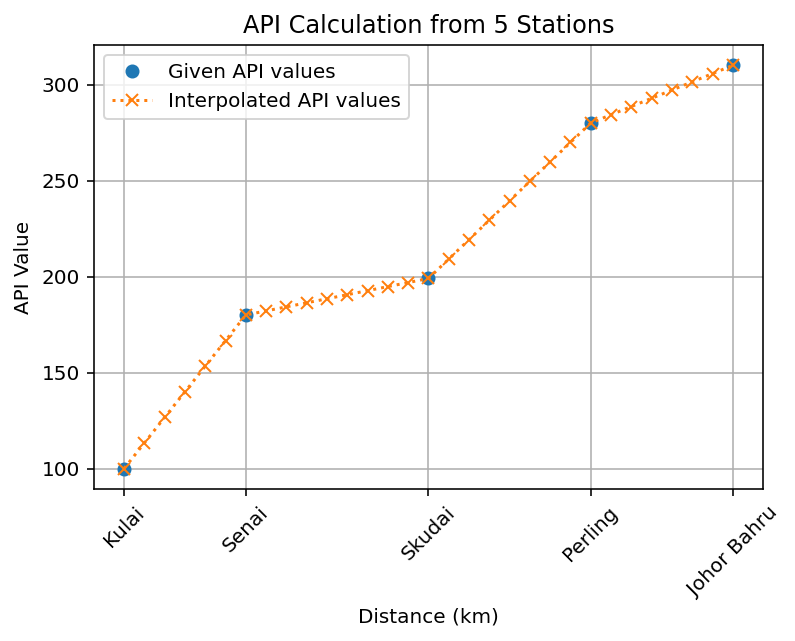
\includegraphics[height=0.56\textheight]{../images/chapter12/api_calculation_plot.png}
    \end{center}
    \small The five known stations (circles) anchor a straight-line
    estimate (dotted) for every kilometre in between.
\end{frame}

%===============================================================================
\section{Increasing Signal Detail}
%===============================================================================

\begin{frame}{Interpolation Applications in Engineering}
    \leavevmode
    Two broad uses recur throughout electrical engineering:
    \begin{itemize}
        \item \alert{Evaluating unknown values} between known points ---
              the API example just shown.
        \item \alert{Increasing the detail (resolution)} of an
              undersampled signal.
    \end{itemize}

    \vspace{3mm}
    \begin{block}{Upsampling}
        Adding points \emph{between} existing samples by interpolation is
        called \alert{upsampling}. It cannot invent information the
        sensor never recorded --- it can only estimate plausible values
        consistent with the samples that exist.
    \end{block}
\end{frame}

\begin{frame}[fragile]{Worked Example: Sharpening an ECG Signal}
    \leavevmode
    \small
    A wireless ECG device under-samples to save energy. Spline
    interpolation adds points between the original samples:

\begin{lstlisting}
reduced_ecg_data = pd.read_csv('reduced_ecg_signal.csv')
time_reduced = reduced_ecg_data['Time(s)'].values
amplitude_reduced = reduced_ecg_data['Amplitude'].values

spline_interpolation = interp1d(time_reduced,
                                 amplitude_reduced, kind='cubic')

new_time_high = np.linspace(time_reduced.min(),
                             time_reduced.max(),
                             len(time_reduced) * 10)
new_amplitude_high = spline_interpolation(new_time_high)
\end{lstlisting}
\end{frame}

\begin{frame}{Before and After: ECG Resolution}
    \leavevmode
    \begin{center}
    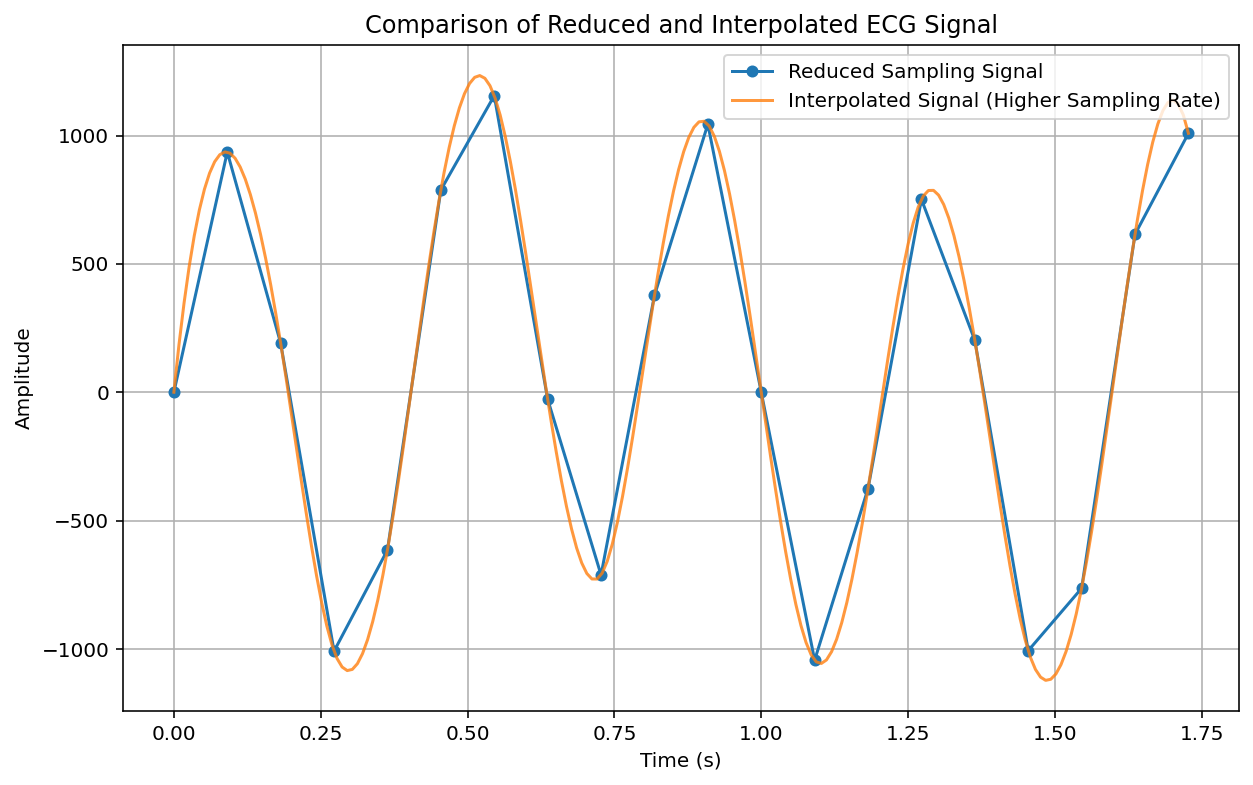
\includegraphics[width=0.62\linewidth]{../images/chapter12/ecg_signal_comparison.png}
    \end{center}
    \small The original 100-point recording (markers) versus the
    10$\times$-upsampled spline interpolation (smooth line) --- the same
    heartbeat, described with far more detail between samples.
\end{frame}

\begin{frame}{Worked Example: DAC Upsampling}
    \leavevmode
    \small
    A digital-to-analog converter (DAC) --- the final step in playing
    digital audio --- benefits from interpolation \emph{before}
    conversion, simplifying the lowpass filter that follows:

    \[
    \text{Audio Signal} \to \text{Interpolation (upsampling)} \to
    \text{Lowpass Filter} \to \text{DAC}
    \]

    \vspace{2mm}
    \begin{itemize}\small
        \item \textbf{Linear}: straight lines between points.
        \item \textbf{Nearest}: step-like, assigns the nearest sample.
        \item \textbf{PCHIP}: smooth, \alert{no overshoot}, preserves
              monotonicity.
        \item \textbf{Spline}: smooth, continuous derivatives, \alert{can}
              overshoot.
    \end{itemize}
\end{frame}

\begin{frame}{Comparing Four Methods on a DAC Signal}
    \leavevmode
    \begin{center}
    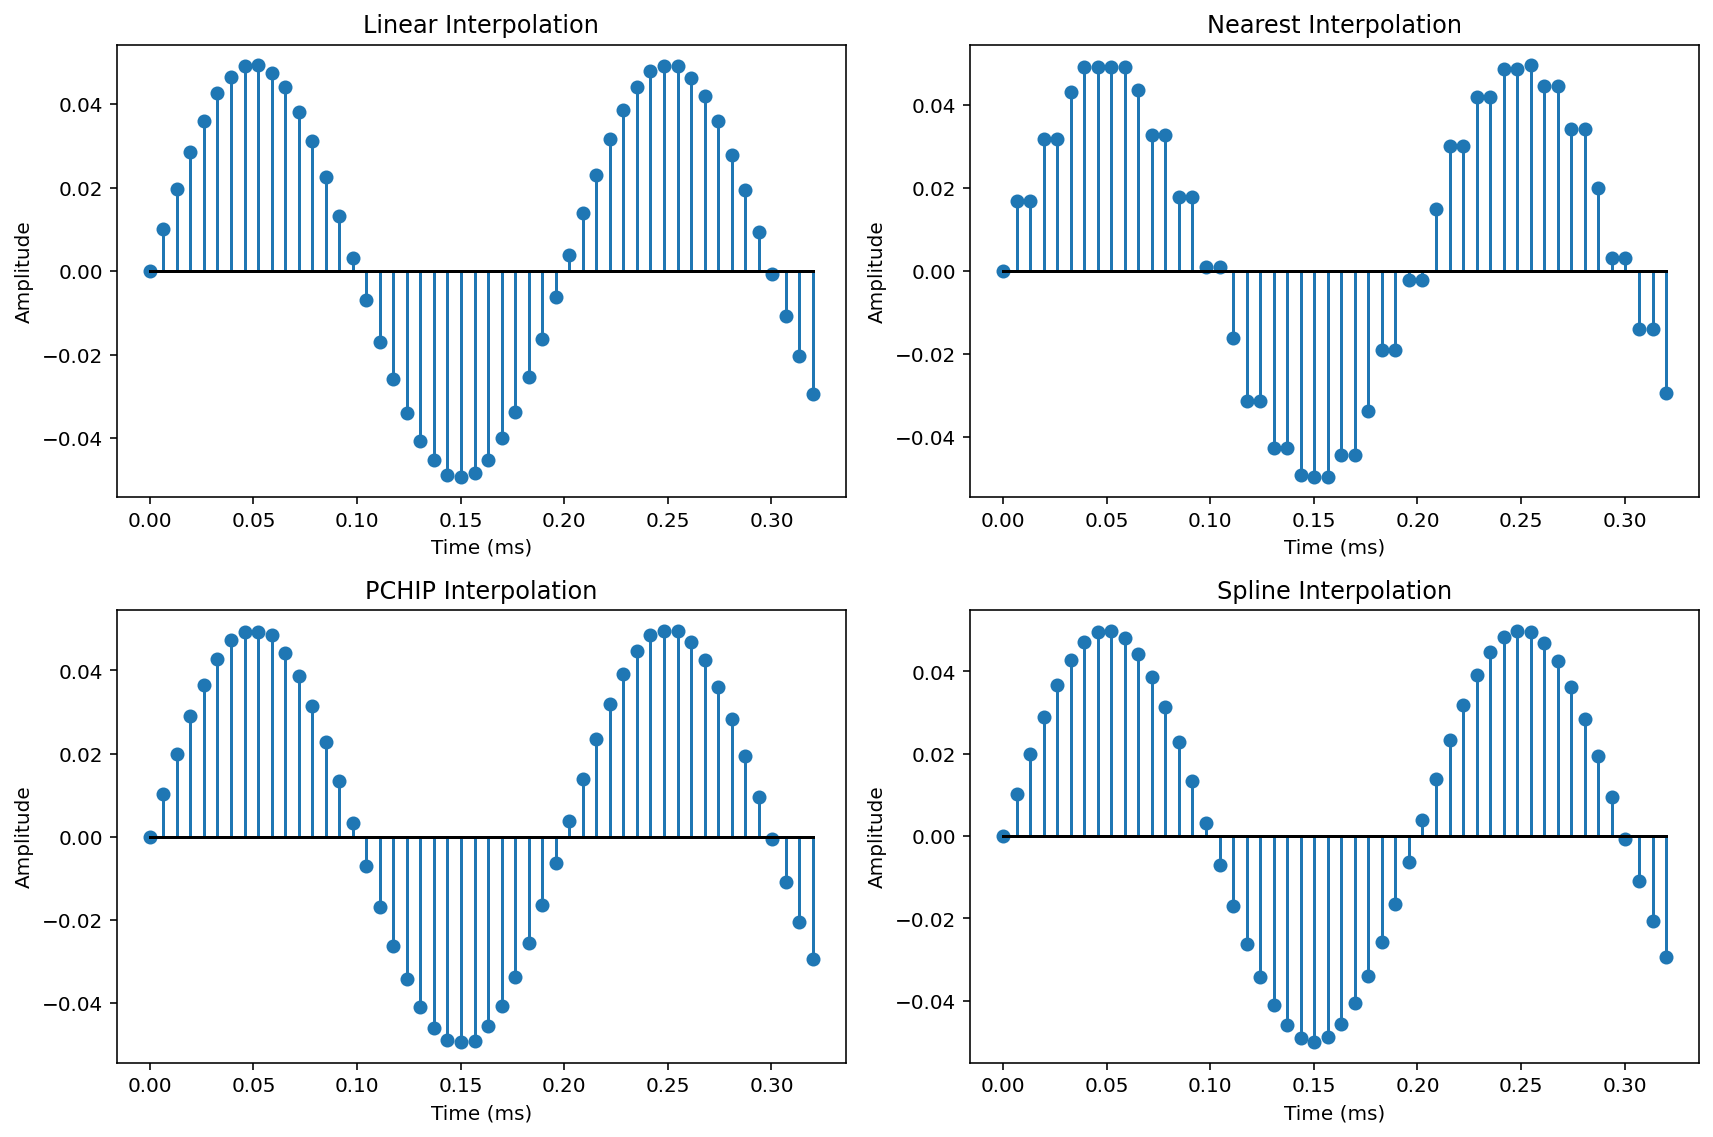
\includegraphics[width=0.56\linewidth]{../images/chapter12/dac_interpolation_methods.png}
    \end{center}
    \small Linear and spline look visually similar; nearest shows the
    characteristic steps; PCHIP tracks the data closely without spline's
    overshoot risk.
\end{frame}

%===============================================================================
\section{Curve Fitting with Polynomials}
%===============================================================================

\begin{frame}[fragile]{A Straight-Line Trendline}
    \leavevmode
    Given scattered, noisy measurements, what single line
    $y = mx + b$ best describes the trend? \texttt{np.polyfit()} answers
    this directly:

\begin{lstlisting}
x = np.array([0, 1, 2, 3, 4, 5])
y = np.array([1.1, 2.9, 5.2, 6.8, 9.3, 11.0])

m, b = np.polyfit(x, y, 1)
print(f"Best-fit line: y = {m:.2f}x + {b:.2f}")

y_fit = np.polyval([m, b], x)
\end{lstlisting}
    \texttt{Best-fit line: y = 1.99x + 1.03}

    \vspace{2mm}
    \small Unlike interpolation, this line does \alert{not} pass through
    any of the original noisy points exactly --- it summarizes the trend.
\end{frame}

\begin{frame}[fragile]{Fitting Higher-Degree Polynomials}
    \leavevmode
    The same \texttt{polyfit}/\texttt{polyval} pair scales to any degree:

\begin{lstlisting}
p = np.polyfit(x, y, 3)  # Fit a 3rd-degree polynomial
y_fit = np.polyval(p, x) # Evaluate it
\end{lstlisting}

    \vspace{2mm}
    \begin{block}{Why model with a polynomial at all?}
        \small Automating a process, analyzing the relationship between
        variables, and identifying trends --- e.g.\ modelling yearly
        climate data or internet-usage growth.
    \end{block}
\end{frame}

\begin{frame}[fragile]{Worked Example: Sensor Calibration}
    \leavevmode
    \small
    A temperature sensor reads in volts over $20$--$50^\circ$C. Find the
    function converting volts to temperature:

\begin{lstlisting}
df = pd.read_excel('sensor_calibration.xlsx')
V, T = df['V'].values, df['T'].values

p = np.polyfit(V, T, 1)   # linear fit
s_t = np.polyval(p, V)
print(f'T(V) = {p[0]:.2f}V + {p[1]:.2f}')
\end{lstlisting}
    \texttt{T(V) = 14.74V + -9.33}

    \vspace{2mm}
    \alert{This is sensor calibration}: one \texttt{polyfit()} call turns
    a raw voltage reading into a trustworthy temperature.
\end{frame}

\begin{frame}{The Calibration Curve}
    \leavevmode
    \begin{center}
    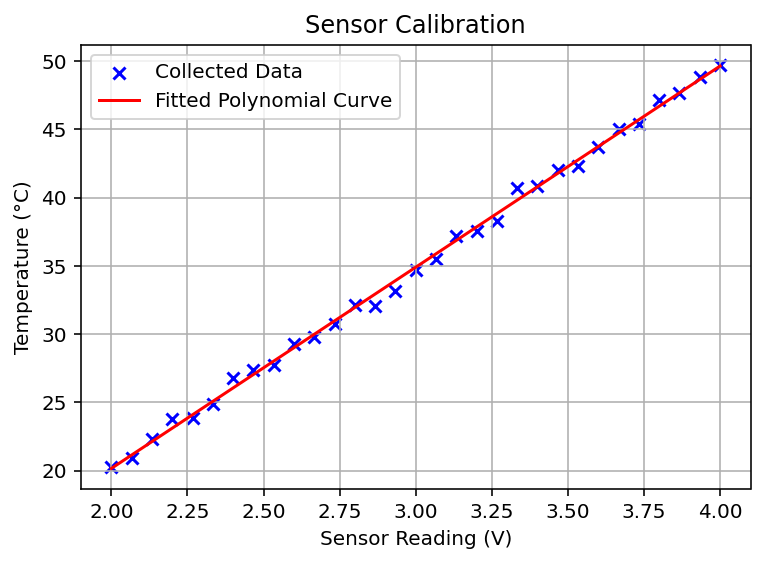
\includegraphics[width=0.5\linewidth]{../images/chapter12/sensor_calibration.png}
    \end{center}
    \small Collected data (crosses) with the fitted linear calibration
    curve $T(V) = 14.74V - 9.33$ (line).
\end{frame}

\begin{frame}{Worked Example: Internet Usage Trend --- the Data}
    \leavevmode
    \small
    Six months of internet usage (hours) for five first-time users. Task:
    find the trend and predict months 7--9.

    \begin{table}
    \centering\scriptsize
    \begin{tabular}{cccccccc}
        \toprule
        \textbf{Person} & M1 & M2 & M3 & M4 & M5 & M6 \\
        \midrule
        1 & 7 & 11 & 23 & 59 & 120 & 180 \\
        2 & 3 & 8  & 20 & 48 & 88  & 140 \\
        3 & 4 & 11 & 21 & 58 & 128 & 195 \\
        \bottomrule
    \end{tabular}
    \end{table}

    \vspace{2mm}
    Fit 1st-, 2nd-, and 3rd-degree polynomials and compare their
    predictions.
\end{frame}

\begin{frame}[fragile]{Fitting Three Degrees at Once}
    \leavevmode
\begin{lstlisting}
months = np.arange(1, 7)
month_matrix = np.tile(months, (data.shape[0], 1))

p1 = np.polyfit(month_matrix.flatten(), data.flatten(), 1)
p2 = np.polyfit(month_matrix.flatten(), data.flatten(), 2)
p3 = np.polyfit(month_matrix.flatten(), data.flatten(), 3)

months_predict = np.array([7, 8, 9])
usage_1 = np.polyval(p1, months_predict)
usage_2 = np.polyval(p2, months_predict)
usage_3 = np.polyval(p3, months_predict)
\end{lstlisting}
    \scriptsize
    \texttt{1st order: [169.7  201.6  233.4]} \quad
    \texttt{2nd order: [244.5  340.5  452.4]} \quad
    \texttt{3rd order: [244.3  340.0  451.4]}
\end{frame}

\begin{frame}{Choosing a Degree: The Plot Tells the Story}
    \leavevmode
    \begin{center}
    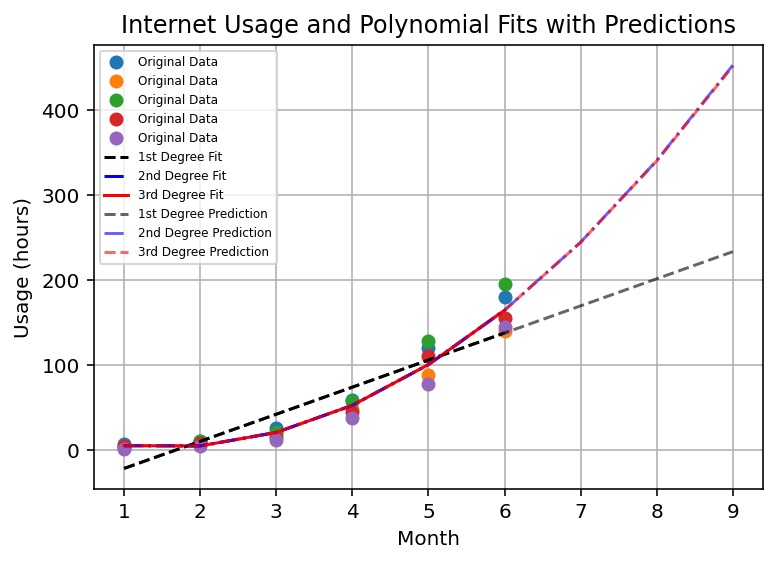
\includegraphics[width=0.56\linewidth]{../images/chapter12/internet_usage_fit.png}
    \end{center}
    \small The 1st-degree (linear) fit substantially
    \alert{underestimates} the accelerating growth. The 2nd- and
    3rd-degree fits track it closely and agree with each other.
\end{frame}

\begin{frame}{Worked Example: Water Usage and $R^2$}
    \leavevmode
    \small
    A farmer wants an automatic irrigation formula from one harvest
    cycle's water-usage data. Which polynomial degree is the right
    choice?

    \vspace{2mm}
    \begin{block}{$R^2$: how much variation the fit explains}
        \[
        R^2 = 1 - \frac{\sum_i (d_i - f_i)^2}{\sum_i d_i^2}
        \]
        $d_i$ = measured data, $f_i$ = fitted data. Closer to $1$ is
        better --- but \alert{not the whole story}.
    \end{block}
\end{frame}

\begin{frame}[fragile]{Computing $R^2$ for Five Degrees}
    \leavevmode
\begin{lstlisting}
N = 5
water_fit = [np.polyval(np.polyfit(day, water, n), day)
             for n in range(1, N + 1)]

R2 = [1 - np.sum((fit - water)**2) / np.sum((water - np.mean(water))**2)
      for fit in water_fit]
\end{lstlisting}

    \vspace{1mm}
    \scriptsize
    \texttt{Order 1 = 0.9743} \quad \texttt{Order 2 = 0.9750} \quad
    \texttt{Order 3 = 0.9947} \quad \texttt{Order 4 = 0.9947} \quad
    \texttt{Order 5 = 0.9961}

    \vspace{2mm}
    \begin{alertblock}{Diminishing returns}
        $R^2$ jumps from $0.975$ to $0.995$ going from order 2 to 3, then
        barely moves beyond that. Order 3 is the sensible choice: good
        accuracy, no unnecessary complexity.
    \end{alertblock}
\end{frame}

\begin{frame}{Why Not Always Pick the Highest $R^2$?}
    \leavevmode
    \begin{center}
    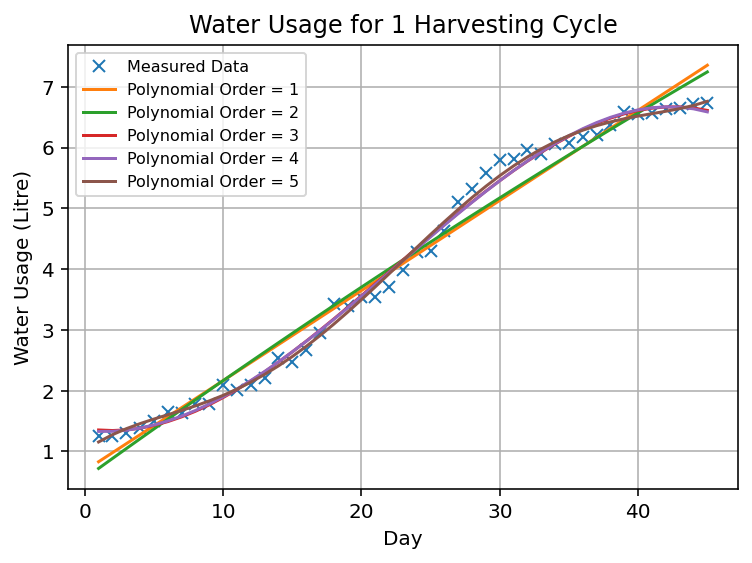
\includegraphics[height=0.44\textheight]{../images/chapter12/water_usage_fit.png}
    \end{center}

    \vspace{1mm}
    \begin{block}{Overfitting}
        \scriptsize A polynomial with enough degrees can track \emph{every
        wiggle} in noisy data, including the noise itself --- it then
        describes only \alert{this particular sample}, and predicts
        poorly on new data.
    \end{block}
\end{frame}

%===============================================================================
\section{EE Focus: The Bench Circuit's Time Constant}
%===============================================================================

\begin{frame}{Back to the Running Dataset}
    \leavevmode
    The nominal time constant of the bench RC circuit is
    $\tau = RC = 0.47\,\text{s}$ --- but that assumes the resistor and
    capacitor are exactly their marked values. Real components carry
    tolerances.

    \vspace{3mm}
    \begin{alertblock}{The honest answer comes from the data}
        What is the \alert{measured} $\tau$, from the actual voltage
        recording? This is curve fitting applied to the chapter's own
        running example.
    \end{alertblock}
\end{frame}

\begin{frame}{The Trick: Logarithms Make It Linear}
    \leavevmode
    $v(t) = V_0 e^{-t/\tau}$ is not a straight line, and
    \texttt{np.polyfit()} fits polynomials. Taking logarithms of both
    sides:

    \[
    \ln v = \ln V_0 - \frac{t}{\tau}
    \]

    \vspace{2mm}
    \begin{block}{This \emph{is} a straight line in $t$}
        Slope $= -1/\tau$, intercept $= \ln V_0$. Fitting a degree-1
        polynomial to $\ln v$ recovers \alert{both} parameters at once.
    \end{block}
\end{frame}

\begin{frame}[fragile]{Recovering $\tau$ from the Data}
    \leavevmode
\begin{lstlisting}
t = np.arange(0, 2.001, 0.02)
v = 12.0 * np.exp(-t / 0.47)   # stands in for measured voltage

slope, intercept = np.polyfit(t, np.log(v), 1)

tau_measured = -1 / slope
V0_measured  = np.exp(intercept)
\end{lstlisting}

    \vspace{1mm}
    \texttt{Fitted slope:  -2.12766 per second}\\
    \texttt{Measured tau:  0.4700 s}\\
    \texttt{Measured V0:   12.0000 V}

    \vspace{2mm}
    \small Three lines of code measure the circuit's \alert{actual}
    $RC$ product, rather than assuming the marked component values.
\end{frame}

\begin{frame}{Two Cautions Worth Carrying Forward}
    \leavevmode
    \begin{block}{1. The logarithm is undefined for $v \le 0$}
        \small Any sample that noise has driven to zero or below must be
        excluded \emph{before} fitting.
    \end{block}

    \vspace{3mm}
    \begin{block}{2. Logarithms distort the error weighting}
        \small They compress large voltages and stretch small ones, so
        the tail of the decay influences the fit more than it would in a
        direct fit. Fine for a first estimate; for precision work, a
        nonlinear fit to the original exponential is the better tool.
    \end{block}
\end{frame}

%===============================================================================
\section{Summary}
%===============================================================================

\begin{frame}{Chapter Summary}
    \leavevmode
    \small
    \begin{itemize}
        \item \textbf{Interpolation} passes exactly through measured
              points; \textbf{curve fitting} finds the best model for a
              noisy whole dataset. Noisy data calls for fitting, not
              interpolation.
        \item \texttt{np.interp()} does linear interpolation directly;
              \texttt{interp1d()} adds \texttt{nearest}, \texttt{cubic},
              and spline methods via \texttt{kind}.
        \item The method must suit the physics: nearest $\to$ steps,
              linear $\to$ corners, cubic/PCHIP $\to$ smooth curves (but
              spline can invent overshoot the data never contained).
        \item \texttt{np.polyfit(x, y, n)} fits a degree-$n$ polynomial;
              \texttt{np.polyval()} evaluates it. Degree 1 is a
              straight-line trendline --- the basis of sensor
              calibration.
        \item $R^2$ measures explained variation, but always rises with
              degree. A polynomial that tracks every wiggle is
              \alert{overfitted} and predicts poorly.
        \item Not every model is a polynomial: an exponential decay
              becomes linear under logarithms, recovering the bench
              circuit's $\tau$ with the same \texttt{polyfit()} tool.
    \end{itemize}
\end{frame}

\begin{frame}{Where This Is Going}
    \leavevmode
    \small
    This chapter answered \emph{what value lies between} (or \emph{near})
    the data you have. The next chapters build on exactly this
    foundation.

    \vspace{3mm}
    \begin{itemize}
        \item Chapter 13: numerical calculus --- derivatives and
              integrals computed directly from arrays, and polynomial
              models of system behaviour.
        \item The bench circuit's measured $\tau$, found here by curve
              fitting, reappears as a check against the calculus-based
              methods in the next chapter.
    \end{itemize}

    \vspace{4mm}
    \begin{center}
        \large\color{primary}\textbf{Next: Numerical Calculus and System Models}
    \end{center}
\end{frame}

\end{document}
